\documentclass[serif, aspectratio=169]{beamer}
%\documentclass[serif]{beamer}  % for 4:3 ratio

\RequirePackage{minted2}
\usepackage[T1]{fontenc} 
\usepackage[utf8]{inputenc}
\usepackage{fourier} % see "http://faq.ktug.org/wiki/uploads/MathFonts.pdf" for other options
\usepackage{hyperref}
\usepackage{latexsym,amsmath,xcolor,multicol,booktabs,calligra}
\usepackage{graphicx,pstricks,listings,stackengine}
\usepackage{lipsum}
\usepackage{../HKUSTstyle}

%imports customs%
\usepackage{caption}    % for subfigures
\usepackage{subcaption} % for subfigures
\usepackage{ragged2e}
\usepackage{booktabs,makecell}
\usepackage{colortbl}
\usepackage{multirow}
\usepackage{cite}
\usepackage{tcolorbox}
\usepackage[sort,authoryear]{natbib}

\author{Julien Bezançon}

\title{Python Programmation}
\subtitle{CM 3~: Functions and Strings}

\institute{julien.bezancon@univ-lorraine.fr / \url{https://julienbez.github.io}}

\date{}

% defs
\def\cmd#1{\texttt{\color{red}\footnotesize $\backslash$#1}}
\def\env#1{\texttt{\color{blue}\footnotesize #1}}

% set colors
\definecolor{hkustyellow}{RGB}{167, 131, 55}
\definecolor{hkustblue}{RGB}{0, 56, 116}
\definecolor{hkustred}{RGB}{209, 51, 59}

\lstset{
    basicstyle=\ttfamily\small,
    keywordstyle=\bfseries\color{deepblue},
    emphstyle=\ttfamily\color{deepred},    % Custom highlighting style
    stringstyle=\color{deepgreen},
    numbers=left,
    numberstyle=\small\color{halfgray},
    rulesepcolor=\color{red!20!green!20!blue!20},
    frame=shadowbox,
}

\begin{document} %  --- --- --- --- --- --- --- --- --- --- --- --- 

\begin{frame}[noframenumbering,plain]
    \titlepage
    \vspace*{-0.6cm}
    \begin{figure}[htpb]
        \begin{center}
            \hspace{0.3cm}
            
\includegraphics[width=0.7\columnwidth]{../../../IMAGES/loria_idmc.png}
        \end{center}
    \end{figure}
\end{frame}

% \begin{frame}    
%     \tableofcontents[sectionstyle=show,
%     subsectionstyle=show/shaded/hide,
%     subsubsectionstyle=show/shaded/hide]
% \end{frame}

\section{Before we start...}

\begin{exoframe}
    \begin{center}
        \Large
        What did you learn during last lecture ? \\
        Any questions ?
    \end{center}
\end{exoframe}

\begin{frame}{Doggy bag}
    \begin{minipage}{0.45\columnwidth}
        \begin{block}{Data structures}
            \begin{itemize}
                \item Lists
                \item Dictionaries
                \item Tuples
                \item Sets
            \end{itemize}
        \end{block}
        \begin{block}{Advanced Python Stuffs}
            \begin{itemize}
                \item Advanced loops
                \item Functions
                % \item Range
            \end{itemize}
        \end{block}
    \end{minipage}
    \hfill
    \begin{minipage}{0.45\columnwidth}
        \begin{figure}
            
\includegraphics[width=0.9\columnwidth]{../../../FIGURES/divers/doggybag.jpg}
        \end{figure}
    \end{minipage}
\end{frame}

\begin{frame}{A quick word about TDs}
    \begin{block}{Last TD}
        \begin{itemize}
            \item Not graded
            \item 1 week before delivery
        \end{itemize}
    \end{block}
    \begin{block}{Next TDs}
        \begin{itemize}
            \item Might be graded
            \item To send at the end of the session !
        \end{itemize}
    \end{block}
    \vspace{15pt}
    \begin{center}
        \Large
        Not doing all exercises is ok. \\ Do what you can.
    \end{center}
\end{frame}

\section{Your First Functions}

\begin{frame}[fragile]{A Simple Function}
    \begin{pythoncode}
    def add_values(param1, param2):
        value = param1 + param2
        return value

    add_values(2,4) # => 6
    \end{pythoncode}
    \begin{block}{}
        \begin{itemize}
            \item Called by using its name
            \item Any number of parameters
            \item Parameters have no explicit type
            \item Returns "None" if no "return" statement
        \end{itemize}
    \end{block}
\end{frame}

\begin{frame}[fragile]{A Function that Returns Multiple Values}
    \begin{pythoncode}
    def add_values(param1, param2):
        value1 = param1 + param2
        value2 = param1 - param2
        value3 = param1 * param2
        return value1, value2, value3

    add_values(2,4) # => 6, -2, 8
    \end{pythoncode}
    \begin{block}{}
        \begin{itemize}
            \item Can return multiple values
            \item In that case, "return" works as a tuple
        \end{itemize}
    \end{block}
\end{frame}

\begin{frame}[fragile]{A Function with a Docstring}
    \begin{pythoncode}
    def add_values(param1, param2):
        """
        Add the values of param1 and param2.

        Args: param1 (int), param2 (int)
        Returns: value (int)
        """
        value = param1 + param2
        return value
    \end{pythoncode}
    \begin{block}{}
        \begin{itemize}
            \item The first string literal inside a function body is a docstring
            \item A docstring is optional but highly recommanded
            \item Used to describe what the function does
        \end{itemize}
    \end{block}
\end{frame}

\section{Parameters and Arguments}

\begin{frame}[fragile]{Basic Parameters}
    \begin{pythoncode}
    def add_values(param1, param2):
        value = param1 + param2
        return value

    add_values(2,4) # => 6
    add_values()
    # => TypeError: add_values() missing 2 required positional 
    #               arguments: 'param1' and 'param2'
    \end{pythoncode}
    \begin{block}{}
        \begin{itemize}
            \item This function has two parameters
            \item These parameters are mandatory, they must be \textbf{specified}
            \item You can add any number of parameters
        \end{itemize}
    \end{block}
\end{frame}

\begin{frame}[fragile]{Default/Named Parameters}
    \begin{pythoncode}
    def add_values(param1,param2,multiplier=5):
        value = (param1 + param2) * multiplier
        return value

    add_values(2,4,multiplier=5)    # => 30
    add_values(2,4)                 # => 30
    add_values(2,4,multiplier=10)   # => 60
    add_values(2,4,10)              # => 60
    \end{pythoncode}
    \begin{block}{}
        \begin{itemize}
            \item You can add a default value to a parameter 
            \item If a parameter is not specified, its default value is used (if it has one)
        \end{itemize}
    \end{block}
\end{frame}

\begin{frame}[fragile]{Arguments}
    \begin{pythoncode}
    def ask_yn(prompt, retries=4, complaint='Enter Y/N!'):
        for i in range(retries):
            ok = input(prompt)
        
            if ok in ('Y', 'y'):
                return True      
            if ok in ('N', 'n'):
                return False
        
        print(complaint)
        return False
    \end{pythoncode}
    \begin{block}{}
        \begin{itemize}
            \item Mandatory argument: "prompt"
            \item Keyword argument: "retries" and "complaint"
        \end{itemize}
    \end{block}
\end{frame}

\begin{frame}[fragile]{Arguments}
    \begin{pythoncode}
    # ask_yn(prompt, retries=4, complaint='...')

    # Call with only the mandatory argument
    ask_yn('Really quit?')

    # Call with one keyword argument
    ask_yn('OK to overwrite the file?', retries=2)

    # Call with one keyword argument - in any order!
    ask_yn('Update status?', complaint='Just Y/N')

    # Call with all of the keyword arguments
    ask_yn('Send text?', retries=2, complaint='Y/N please!')
    \end{pythoncode}
\end{frame}

\begin{frame}[fragile]{The Dead Parrot Example}
    \begin{pythoncode}
    def parrot(voltage, state='a stiff', action='voom',
               type='Norwegian Blue'):
        print("-- This parrot wouldn't", action, end=' ')
        print("if you put", voltage, "volts through it.")
        print("-- Lovely plumage, the", type)
        print("-- It's", state, "!")
    \end{pythoncode}
    \begin{block}{}
        \begin{itemize}
            \item What does this fuction do ?
        \end{itemize}
    \end{block}
\end{frame}

\begin{frame}[fragile]{Dead Parrot: Valid Calls}
    \begin{pythoncode}
    # def parrot(voltage, state='…', action='…', type='…')

    # 1 positional argument
    parrot(1000)
    # 1 keyword argument
    parrot(voltage=1000)
    # 2 keyword arguments
    parrot(voltage=1000000, action='VOOOOOM')
    # 2 keyword arguments
    parrot(action='VOOOOOM', voltage=1000000)
    # 3 positional arguments
    parrot('a million', 'bereft of life', 'jump')
    \end{pythoncode}
\end{frame}


\begin{frame}[fragile]{Dead Parrot: Invalid Calls}
    \begin{pythoncode}
    # def parrot(voltage, state='…', action='…', type='…')

    # required argument missing
    parrot()
    # non-keyword argument after a keyword argument
    parrot(voltage=5.0, 'dead')
    # duplicate value for the same argument
    parrot(110, voltage=220)
    # unknown keyword argument
    parrot(actor='John Cleese')
    \end{pythoncode}
\end{frame}

\begin{frame}[fragile]{Other Examples of Keyword Arguments}
    \begin{pythoncode}
    print("hello", sep=' ', end='\n', file=sys.stdout, flush=False)
    range(start, stop, step=1)
    enumerate(iter, start=0)
    int(x, base=10)
    seq.sort(*, key=None, reverse=None)

    subprocess.Popen(args, bufsize=-1, executable=None,
    stdin=None, stdout=None, stderr=None, preexec_fn=None,
    close_fds=True, shell=False, cwd=None, env=None,
    universal_newlines=None, startupinfo=None,
    creationflags=0, restore_signals=True,
    start_new_session=False, pass_fds=(), encoding=None,
    errors=None, text=None)
    \end{pythoncode}
\end{frame}

\begin{frame}[fragile]{A Weird Case: Mutable default parameter values}
    \begin{pythoncode}    
    def my_funct(my_list = []):
        my_list.append("hello")
        return my_list

    my_funct([1,2,3]) # => [1,2,3,"hello"]
    my_funct() # => ["hello"], but what happens if I repeat this line ?
    my_funct() # => ?
    my_funct() # => ?
    \end{pythoncode}
    \begin{block}{}
        \begin{itemize}
            \item What happen if I repeat "my\_funct()" several times ?
            \item Why does this happen ?
        \end{itemize}
    \end{block}
\end{frame}

\begin{frame}[fragile]{A Weird Case: Explanation}
    \begin{pythoncode}
    def my_funct(my_list = []):
        print(id(my_list))
        my_list.append("hello")
        return my_list
    
    my_funct() # => 140095566958408, ["hello"]
    my_funct() # => 140095566958408, ["hello","hello"]
    my_funct() # => 140095566958408, ["hello","hello","hello"]
    \end{pythoncode}
    \begin{block}{}
        \begin{itemize}
            \item Default parameters values are defined only once, at function definition
            \item Each new call points to the same object
        \end{itemize}
    \end{block}
\end{frame}

\section{Variadic Arguments}

\begin{frame}[fragile]{Variadic Positional Arguments}
    \begin{pythoncode}
    def product(*nums, scale=1):
        p = scale
        for n in nums:
            p *= n
        return p

    product(3,5) # => 15
    product(3,4,2) # => 24
    product(3,5,scale=10) # => 150
    \end{pythoncode}
    \vspace{10pt}
    \begin{itemize}
        \item A parameter of form "*arg" captures excess arguments
        \item These arguments are stored into the "arg" tuple
        \item Parameters after "*args" must be default/named ones !
    \end{itemize}
    \vspace{10pt}
    \begin{pythoncode}
    print(*objects, sep=' ', end='\n', file="toto.txt", flush=False)
    \end{pythoncode}
\end{frame}

\begin{frame}[fragile]{Unpacking Variadic Positional Arguments}
    \begin{pythoncode}
    def product(*nums, scale=1):
        p = scale
        for n in nums:
            p *= n
        return p

    numbers = [1,2,3,4,5,6]
    product(*numbers) # equivalent to product(1,2,3,4,5,6)
    \end{pythoncode}
    \begin{block}{}
        \begin{itemize}
            \item The syntax "*seq" unpack a sequence into its constituent components
        \end{itemize}
    \end{block}
\end{frame}

\begin{frame}[fragile]{Variadic Keyword Arguments}
    \begin{pythoncode}
    def authorize(quote, **speaker_info):
        print(">", quote)
        print("-" * (len(quote) + 2))
        for k, v in speaker_info.items():
        print(k, v, sep=': ')

    authorize("If music be the food of love, play on.",
              playwright="Shakespeare",act=1,scene=1,
              speaker="Duke Orsino")
    \end{pythoncode}
    \begin{block}{}
        \begin{itemize}
            \item A parameter of form "**kwargs" captures all excess keyword arguments
            \item These arguments are stored into the "kwargs" dictionary
        \end{itemize}
    \end{block}
\end{frame}

\begin{frame}[fragile]{Unpacking Variadic Keyword Arguments}
    \begin{pythoncode}
    authorize("If music be the food of love, play on.",
               playwright="Shakespeare",act=1,scene=1,
               speaker="Duke Orsino")

    # > If music be the food of love, play on.
    # ----------------------------------------
    # act: 1
    # scene: 1
    # speaker: Duke Orsino
    # playwright: Shakespeare
    \end{pythoncode}
\end{frame}

\begin{frame}[fragile]{Variadic Keyword Arguments}
    \begin{pythoncode}
    info = {
        'sonnet': 18,
        'line': 1,
        'author': "Shakespeare"
    }

    authorize("Shall I compare thee to a summer's day", **info)

    # > Shall I compare thee to a summer's day
    # ----------------------------------------
    # line: 1
    # sonnet: 18
    # author: Shakespeare
    \end{pythoncode}
\end{frame}

\section{Python Scope}

\begin{frame}[fragile]{Variables in Functions}
    \begin{pythoncode}
    def add_values(param1, param2):
        value = param1 + param2
        return value

    print(value) # => NameError: name 'value' is not defined.
    \end{pythoncode}
    \pause
    \begin{block}{}
        \begin{itemize}
            \item Variables defined inside a function only work in said function
            \item A variable is only available from inside the region it is created
        \end{itemize}
    \end{block}
\end{frame}

\begin{frame}{The LEGB rule}
    \begin{block}{When Python look up variable names, it does it in this order~:\footnote{\url{https://www.w3schools.com/python/python_scope.asp}}}
        \begin{itemize}
            \item[1.] Local - inside the current function
            \item[2.] Enclosing - inside enclosing functions
            \item[3.] Global - at the top level of the module
            \item[4.] Built-in - in Python's built-in namespace
        \end{itemize}
    \end{block}
\end{frame}

\begin{frame}[fragile]{Local Scope}
    \begin{pythoncode}
    def add_values(param1, param2):
        value = param1 + param2
        return value

    print(value) # => NameError: name 'value' is not defined.
    \end{pythoncode}
    \begin{block}{}
        \begin{itemize}
            \item "value" is only available in the "add\_values" function
            \item "value" does not exist outside of the "add\_values" function
        \end{itemize}
    \end{block}
\end{frame}

\begin{frame}[fragile]{Enclosing Scope}
    \begin{pythoncode}
    def add_values(param1, param2):
        value = param1 + param2
        def show_value():
            print(value)
        show_value()

    add_values(2,4) # => 6
    \end{pythoncode}
    \begin{block}{}
        \begin{itemize}
            \item "value" can be accessed from a function within the "add\_values" function
            \item Why ? Because "show\_value" is \textbf{inside} the "add\_values" function
        \end{itemize}
    \end{block}
\end{frame}

\begin{frame}[fragile]{Global Scope}
    \begin{pythoncode}
    value = 300

    def show_value():
        print(value)

    show_value() # => 300
    \end{pythoncode}
    \begin{block}{}
        \begin{itemize}
            \item Variables created outside of a function can be used by anyone
            \item Variables created outside of a function == global scope
        \end{itemize}
    \end{block}
\end{frame}

\begin{frame}{Built-in Scope}
    \begin{block}{Built-ins are always available and have an usage}
        \begin{itemize}
            \item int(), bool(), str(), float(), etc
            \item print(), zip(), input(), etc
            \item sorted(), min(), max(), len(), etc
        \end{itemize}
    \end{block}
    \vspace{15pt}
    \begin{center}
        \Large
        Built-ins are always available.
    \end{center}
\end{frame}

\begin{frame}{Scopes Summary}
    \begin{minipage}{0.45\columnwidth}
        \begin{figure}
            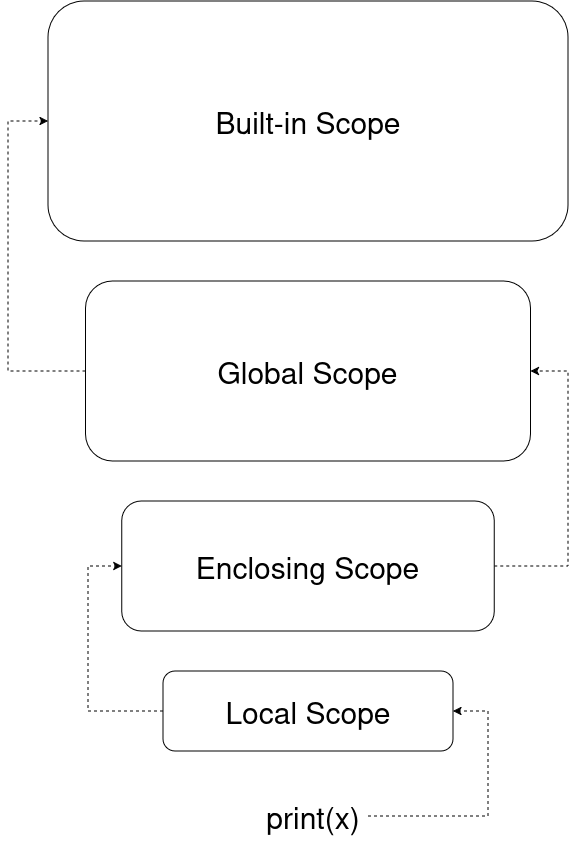
\includegraphics[width=0.75\columnwidth]{../../../FIGURES/python/python_scopes.png}
        \end{figure}
    \end{minipage}
    \begin{minipage}{0.45\columnwidth}
        \begin{block}{Python checks scopes in this order~:}
            \begin{itemize}
                \item[1.] Local scope
                \item[2.] Enclosing scope
                \item[3.] Global scope
                \item[4.] Built-in scope
                \vspace{15pt}
                \item If "x" not found, return an error
            \end{itemize}
        \end{block}
    \end{minipage}
\end{frame}

\begin{frame}[fragile]{Almost Everything is Global Scope}
    \begin{pythoncode}
    success = True

    if success:
        desc = "winner!"
    else:
        desc = "loser"

    print(desc)
    \end{pythoncode}
    \begin{block}{}
        \begin{itemize}
            \item Only functions may define a new scope (local or enclosing)
            \item Other statements and loops does not define new scopes
        \end{itemize}
    \end{block}
\end{frame}

\begin{frame}
    
\end{frame}

\end{document}
